\documentclass[tikz,border=3pt]{standalone}
\usepackage[utf8]{inputenc}
\usepackage[T1]{fontenc}
\usepackage{libertinus}
\usepackage{amsmath,amssymb}
\usetikzlibrary{arrows.meta,calc,patterns,decorations.pathmorphing,decorations.markings,decorations.pathreplacing,bending}
\definecolor{UGblue}{RGB}{0,51,102}
\newcommand{\dbar}{\mathchar'26\mkern-12mu d}
\tikzset{
  >=Stealth,
  every node/.style={font=\small},
  caja/.style={draw,line width=0.9pt},
  pared/.style={draw,line width=1.6pt},
  ejes/.style={->,line width=0.8pt},
  adia/.style={draw,pattern=north east lines,pattern color=black!70,line width=0.5pt},
  gas/.style={fill=UGblue!8},
  punto/.style={fill,circle,inner sep=1.3pt},
  onda/.style={decorate,decoration={snake,amplitude=1.1pt,segment length=5pt,post length=3pt,pre length=0pt}},
}
\begin{document}
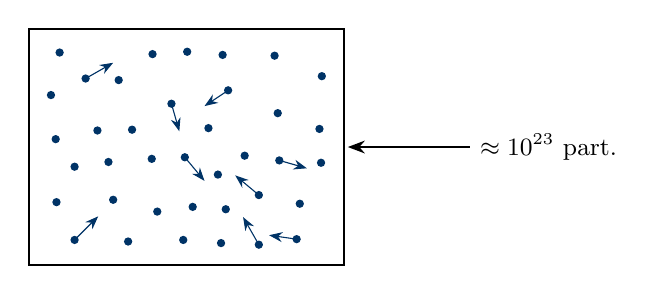
\begin{tikzpicture}
  \draw[caja] (0,0) rectangle (4,3);
  \fill[UGblue] (0.72,2.37) circle (1.5pt);
  \fill[UGblue] (2.92,0.89) circle (1.5pt);
  \fill[UGblue] (1.98,1.37) circle (1.5pt);
  \fill[UGblue] (2.53,2.22) circle (1.5pt);
  \fill[UGblue] (0.58,0.32) circle (1.5pt);
  \fill[UGblue] (3.18,1.33) circle (1.5pt);
  \fill[UGblue] (2.92,0.26) circle (1.5pt);
  \fill[UGblue] (1.81,2.05) circle (1.5pt);
  \fill[UGblue] (3.40,0.33) circle (1.5pt);
  \fill[UGblue] (0.34,1.60) circle (1.5pt);
  \fill[UGblue] (1.01,1.31) circle (1.5pt);
  \fill[UGblue] (0.35,0.80) circle (1.5pt);
  \fill[UGblue] (1.07,0.83) circle (1.5pt);
  \fill[UGblue] (1.26,0.30) circle (1.5pt);
  \fill[UGblue] (2.50,0.71) circle (1.5pt);
  \fill[UGblue] (3.72,2.40) circle (1.5pt);
  \fill[UGblue] (3.16,1.93) circle (1.5pt);
  \fill[UGblue] (1.31,1.72) circle (1.5pt);
  \fill[UGblue] (1.56,1.35) circle (1.5pt);
  \fill[UGblue] (1.96,0.32) circle (1.5pt);
  \fill[UGblue] (3.69,1.73) circle (1.5pt);
  \fill[UGblue] (1.63,0.68) circle (1.5pt);
  \fill[UGblue] (2.01,2.71) circle (1.5pt);
  \fill[UGblue] (0.87,1.71) circle (1.5pt);
  \fill[UGblue] (1.14,2.35) circle (1.5pt);
  \fill[UGblue] (2.74,1.39) circle (1.5pt);
  \fill[UGblue] (3.12,2.66) circle (1.5pt);
  \fill[UGblue] (3.44,0.78) circle (1.5pt);
  \fill[UGblue] (3.71,1.30) circle (1.5pt);
  \fill[UGblue] (1.57,2.68) circle (1.5pt);
  \fill[UGblue] (2.28,1.74) circle (1.5pt);
  \fill[UGblue] (0.39,2.70) circle (1.5pt);
  \fill[UGblue] (0.58,1.25) circle (1.5pt);
  \fill[UGblue] (2.46,2.67) circle (1.5pt);
  \fill[UGblue] (2.08,0.74) circle (1.5pt);
  \fill[UGblue] (0.28,2.16) circle (1.5pt);
  \fill[UGblue] (2.44,0.28) circle (1.5pt);
  \fill[UGblue] (2.40,1.15) circle (1.5pt);
  \draw[->,line width=0.4pt,UGblue] (0.72,2.37) -- ++(0.35,0.20);
  \draw[->,line width=0.4pt,UGblue] (2.92,0.89) -- ++(-0.30,0.25);
  \draw[->,line width=0.4pt,UGblue] (1.98,1.37) -- ++(0.25,-0.30);
  \draw[->,line width=0.4pt,UGblue] (2.53,2.22) -- ++(-0.30,-0.20);
  \draw[->,line width=0.4pt,UGblue] (0.58,0.32) -- ++(0.30,0.30);
  \draw[->,line width=0.4pt,UGblue] (3.18,1.33) -- ++(0.35,-0.10);
  \draw[->,line width=0.4pt,UGblue] (2.92,0.26) -- ++(-0.20,0.35);
  \draw[->,line width=0.4pt,UGblue] (1.81,2.05) -- ++(0.10,-0.35);
  \draw[->,line width=0.4pt,UGblue] (3.40,0.33) -- ++(-0.35,0.05);
  \draw[->,line width=0.7pt] (5.6,1.5) node[right] {$\approx 10^{23}$ part.} -- (4.05,1.5);
\end{tikzpicture}
\end{document}
